\documentclass[11pt]{article}
\usepackage[a4paper, margin=2cm]{geometry} % 设置页面大小为A4,边距为2cm
\usepackage{helvet} % 使用Helvetica(Arial的近似)字体
\usepackage{fancyhdr} % 自定义页眉页脚
\usepackage{graphicx} % 图片插入宏包
\usepackage{amsmath} % 数学公式宏包

\renewcommand{\familydefault}{\sfdefault} % 将默认字体设置为sans serif,类似Arial

% 设置页眉和页脚
\pagestyle{fancy}
\fancyhf{} % 清除默认的页眉和页脚
\lhead{LH Computer Vision and Imaging (30213, 32578, 30241, 37854)} % 在左上角添加学生ID
\rhead{Student ID: 2272583} % 在右上角添加模块代码
\cfoot{\thepage} % 页脚中间显示页码

% 限制文档长度为3页
\usepackage{lipsum} % 生成示例文本的宏包
\usepackage{afterpage}
\usepackage{etoolbox}
\newcounter{pagecount}
\preto{\newpage}{\ifnum\value{pagecount}<3\relax\stepcounter{pagecount}\else\clearpage\fi}

\begin{document}

\section*{Task 1: Laplacian of Gaussian}

\begin{figure}[h]
    \centering
    \begin{minipage}{0.3\textwidth}
        \centering
        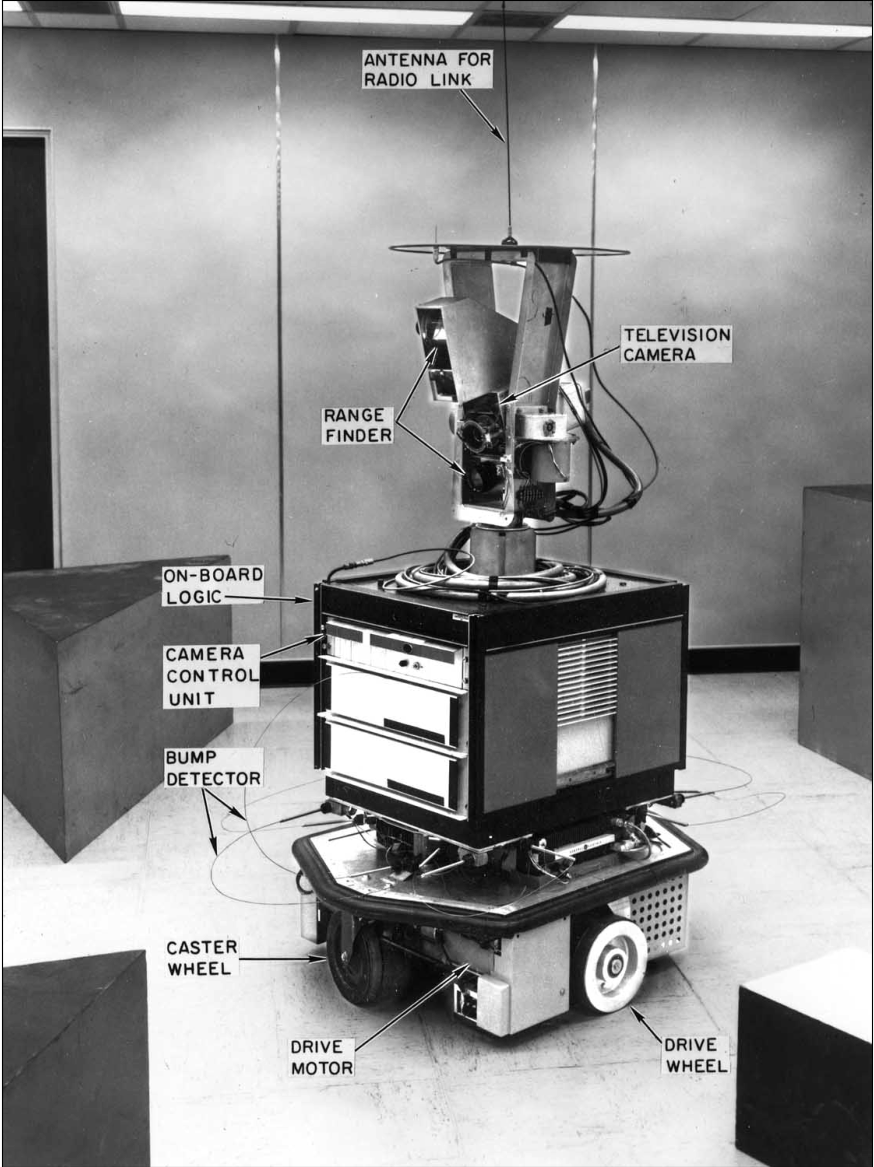
\includegraphics[width=\linewidth]{../img/shakey_original.png}
    \end{minipage}\hfill
    \begin{minipage}{0.3\textwidth}
        \centering
        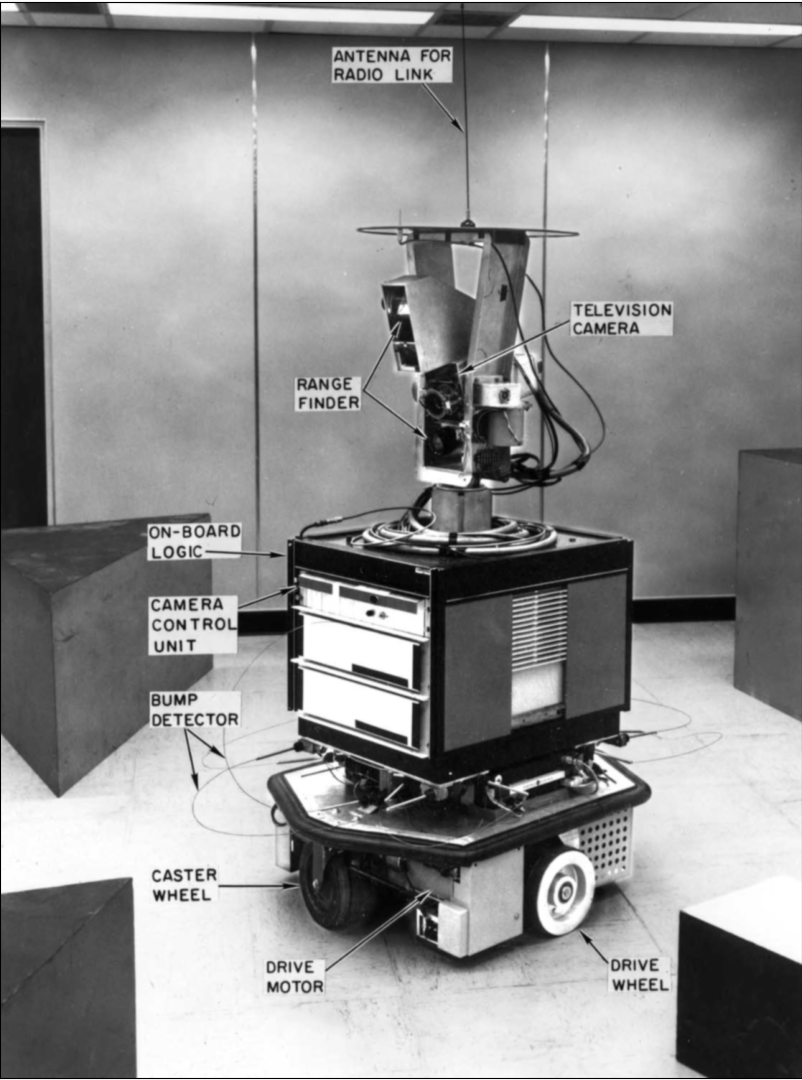
\includegraphics[width=\linewidth]{../img/shakey_smoothed.png}
    \end{minipage}\hfill
    \begin{minipage}{0.3\textwidth}
        \centering
        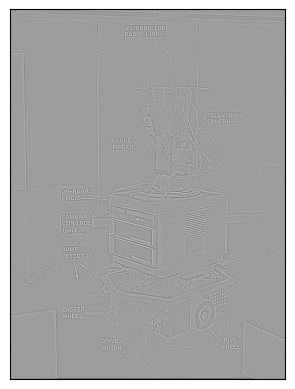
\includegraphics[width=\textwidth]{../img/shakey_log_no_threshold.png}
    \end{minipage}\hfill
\end{figure}

\begin{enumerate}
    \item Generation of the LoG mask with a chosen size and standard deviation.
    \item Convolution of the smoothed image with the LoG mask to highlight edges.
\end{enumerate}

\subsubsection*{Results and Discussion}
The images clearly show the effectiveness of the LoG filter in edge detection. The Gaussian smoothing successfully suppressed the noise, and the log filter successfully extracted the edges of the 'Shakey' image and generated a 'gray' image. . 

\subsubsection*{Noise Removal Technique}
The Gaussian smoothing step serves as a noise removal technique, as it helps to suppress high-frequency noise which could be falsely detected as edges by the LoG filter. 

\section*{Task 2: Edge Detection}

\subsubsection*{Edge Detectors}

\begin{figure}[h]
    \centering
    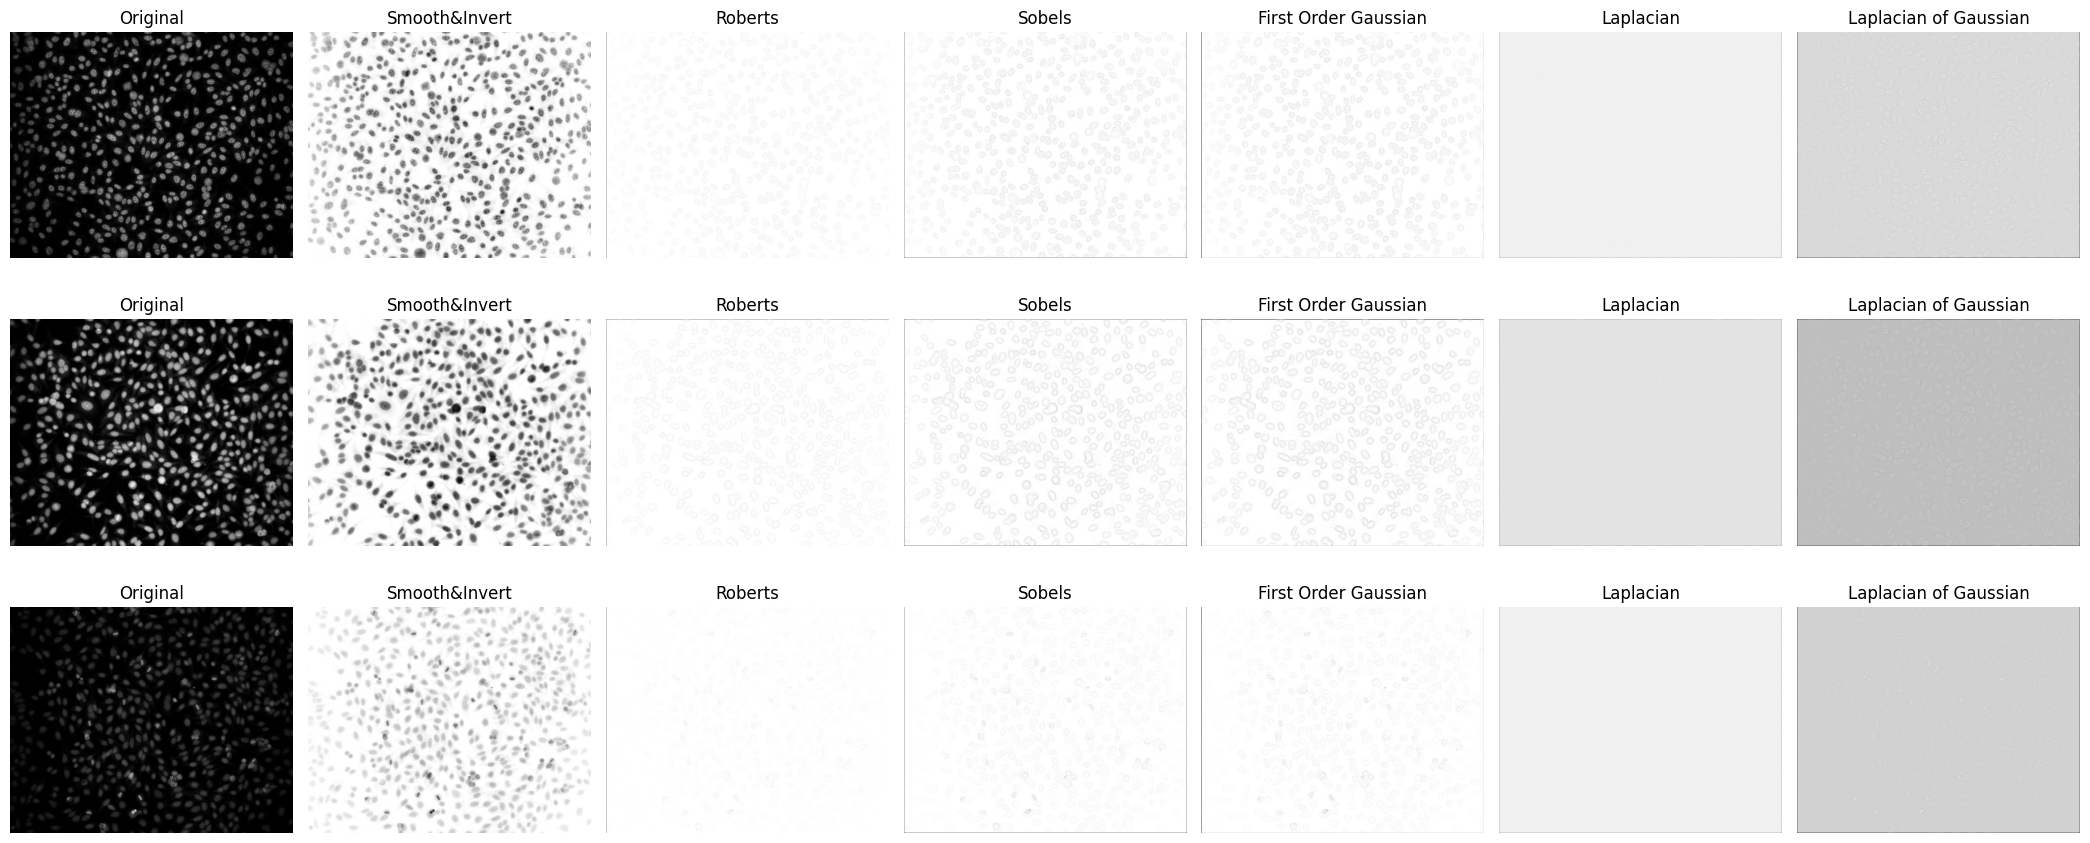
\includegraphics[width=\textwidth]{../img/task2_cells.png}
\end{figure}

\subsubsection*{Roberts}
\begin{enumerate}
    \item The input image is convolved with two 2x2 Roberts cross kernels to compute the gradient components in the x and y directions.
    \item The magnitude of the gradient is calculated, combining both directional components to highlight edges.
\end{enumerate}

\subsubsection*{Sobel}
\begin{enumerate}
    \item The input image is convolved with a pair of 3x3 Sobel kernels to compute the gradient components along the x and y axes.
    \item The gradient magnitudes are combined to form the final edge magnitude image.
\end{enumerate}

\subsubsection*{First Order Gaussian}
\begin{enumerate}
    \item A one-dimensional first-order Gaussian mask is generated based on the provided standard deviation and mean.
    \item The image is convolved with this mask in both the horizontal and vertical directions to calculate the gradients.
    \item The magnitude of the gradient is computed, highlighting the edges.
\end{enumerate}

\subsubsection*{Laplacian}
\begin{enumerate}
    \item The input image is convolved with a 3x3 Laplacian kernel to compute second-order derivatives.
    \item The result of this convolution highlights regions of rapid intensity change.
\end{enumerate}

\subsubsection*{Laplacian of Gaussian (LoG)}
\begin{enumerate}
    \item A Laplacian of Gaussian mask is generated based on the chosen standard deviation and size.
    \item The image is convolved with this LoG mask to apply Gaussian smoothing and then to compute the Laplacian for edge detection.
\end{enumerate}


\subsubsection*{Results and Discussion}
\begin{itemize}
    \item The \textbf{Roberts} filter shows improved edge sensitivity and clarity against the background.
    \item The \textbf{Sobel} filter benefits from Gaussian pre-processing, yielding thicker, more prominent edges with fewer false positives.
    \item The \textbf{First Order Gaussian} filter: While it reduces noise artifacts effectively, there is a potential trade-off in the loss of fine details within the cell structures.
    \item The \textbf{Laplacian} filter: The edges detected are less defined, and the method may fail to capture finer edge details accurately.
    \item The \textbf{Laplacian of Gaussian (LoG)} filter: It can result in an over-smoothing of some areas, potentially obfuscating important subtle features within the cells.
\end{itemize}

\subsubsection*{Noise Removal Technique}
Prior to edge detection, Gaussian filtering was applied to the images as a noise reduction technique. Although Gaussian filtering tends to lower the precision of edge detection, as it can blur the edges slightly, it can ensure that the actual edges are more prominent and noise artifacts are reduced. 

\section*{Task 3: Advanced Edge Detection(Canny)}

\begin{figure}[h]
    \centering
    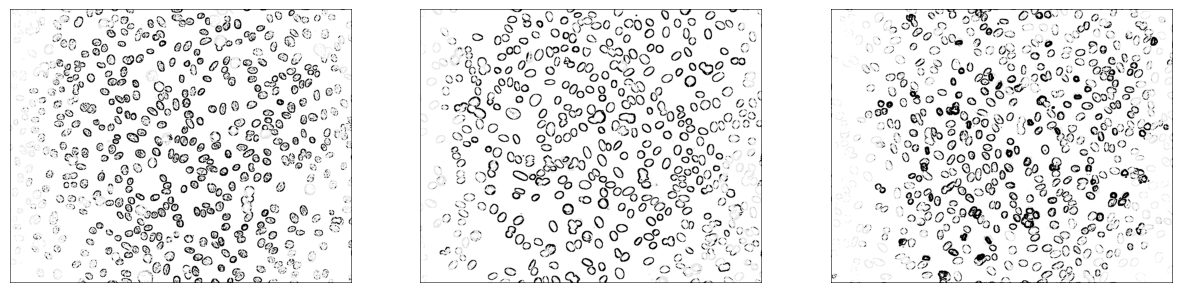
\includegraphics[width=\textwidth]{../img/task3_canny.png}
\end{figure}

\begin{enumerate}
    \item The Gaussian filter is applied to detect gradients and highlight edges by recognizing intensity variations.
    \item Gradients from both directions are merged to measure edge intensity.
    \item Gradient intensity is then thresholded to separate true edges from noise.
\end{enumerate}

\subsubsection*{Results and Discussion}
The application of the Canny Edge Detector resulted in images with clearly defined edges, showing strong gradients where the original images exhibit significant changes in intensity. 

\subsubsection*{Comparison with Canny Edge Detector}
The Canny algorithm's use of double thresholding, more connected edge maps, making it superior for applications requiring high precision in edge detection. But it also results the thicker edges.

\section*{Task 4: Result evaluation}

\begin{figure}[h]
    \centering
    \begin{minipage}{0.3\textwidth}
        \centering
        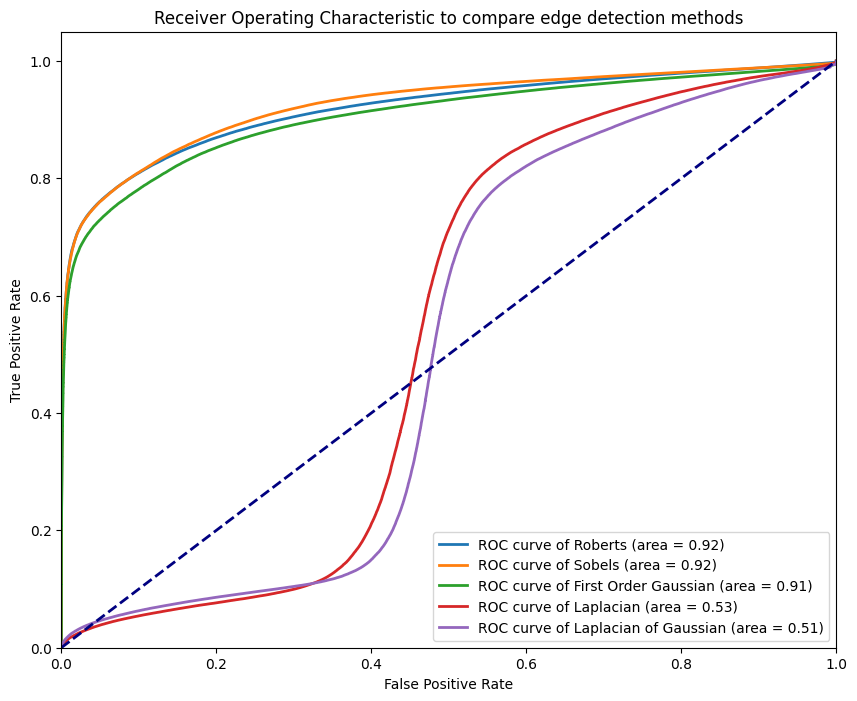
\includegraphics[width=\linewidth]{../img/task4_ROC1.png}
    \end{minipage}\hfill
    \begin{minipage}{0.3\textwidth}
        \centering
        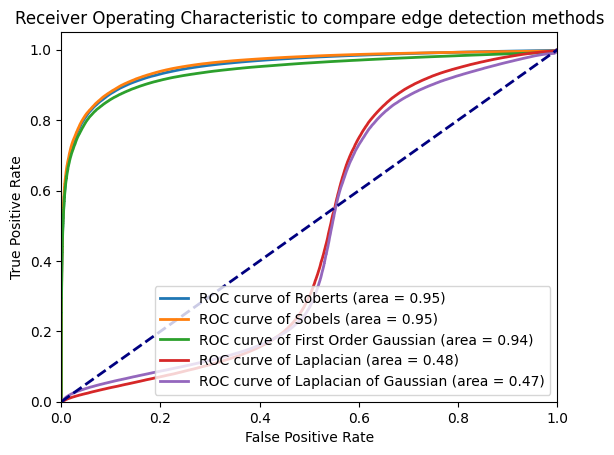
\includegraphics[width=\linewidth]{../img/task4_ROC2.png}
    \end{minipage}\hfill
    \begin{minipage}{0.3\textwidth}
        \centering
        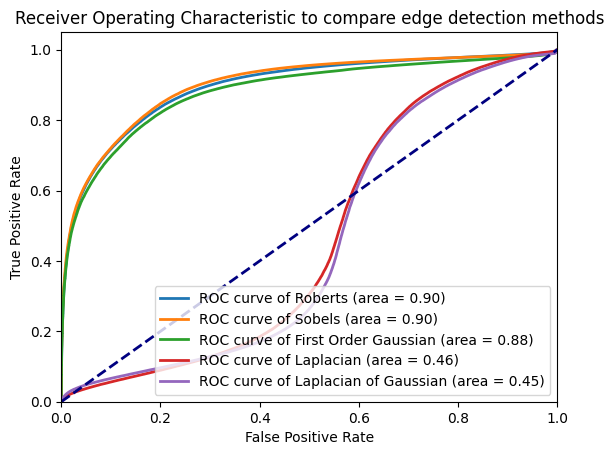
\includegraphics[width=\textwidth]{../img/task4_ROC3.png}
    \end{minipage}\hfill
\end{figure}

\begin{itemize}
    \item Roberts and Sobel have the highest AUC, indicating good sensitivity and specificity.
    \item The First Order Gaussian also performs well, suggesting effective edge detection.
    \item The Laplacian and Laplacian of Gaussian methods have lower AUC values, showing that these methods may have a higher rate of false positives or false negatives.
\end{itemize}

These results suggest that the Roberts and Sobel edge detectors provide more accurate edge detection for the given images when compared to the Laplacian methods in cell detections.The edge detection based on gradient changes may produce more noise in the cell image, resulting in lower AUC values.

\end{document}
